\documentclass[12pt,letterpaper]{article}
\usepackage{graphicx}
\usepackage{tikz}
\usepackage{amsmath}
\usepackage{pdfsync}
\usepackage{url}
\usepackage{hyperref}
\usepackage{microtype}
\usepackage{siunitx}

\hypersetup{colorlinks=true, urlcolor=blue, citecolor=black, linkcolor=black}
\urlstyle{same}

\renewcommand{\d}{\mathrm{d}}

\title{Learning to Use Latex}
\author{Used with permission from Randy McDermott}
\date{\today}

\begin{document}

\maketitle

\section{Introduction}
\label{sec:intro}

The purpose of this document is to provide most of the examples you will need to create a mathematical writeup using \LaTeX.  Simply copy and delete as needed.  The next section gives a quick overview of the document layout and shows how to reference sections of the document.  If you are new to \LaTeX, you will quickly come to appreciate the power of the referencing system.  Indeed, this is the primary reason---together with the quality of the mathematical formulae---that people come to like the \LaTeX~type-setting environment so much more than the wysiwyg (what you see is what you get) environment of Word.  You can easily shuffle sections, equations, figures, and bibliographic references without giving a nanosecond of thought to rearranging the numbers.  It's all done automatically.

% Notice the ~ between \LaTeX and type-setting.  Sometimes this is needed if the spacing looks off in the pdf.  You can also use this after abbreviations within a sentence, because the period makes LaTeX think a new sentence is coming and it will space things differently.  So, for example, Prof.~Trouv\'e would be better than Prof. Trouv\'e.

While this template will hopefully answer most of your questions, you should be aware that the online support for \LaTeX~is amazing.  A quick Google search with \verb=latex= as one of the arguments will return a wealth of information.  At this point, just about anything you can dream up has been done.

\section{Frontmatter}
\label{sec:front}

In \LaTeX~parlance, ``frontmatter'' refers to values set before the \verb=\begin{Document}= command.  For our purposes, this is pretty much self expanatory: change the title and the author name and you should be good.

\section{Section Headings}
\label{sec:layout}
This section shows the various section levels available for the article class.  Each section or subsection can be ``labeled'' and referenced later in the document.  For example, this section is created using the following lines:
\begin{verbatim}
\section{Section Headings}
\label{sec:layout}
\end{verbatim}
To reference this section, use Section \verb=\ref{sec:layout}=, which produces Section \ref{sec:layout}.

Paragraphs are separated by skipping a line in your text editor.  For example,
\begin{verbatim}
...which produces Section \ref{sec:layout}.

Paragraphs are separated by...
\end{verbatim}

If you want to skip lines in your text document but do not want a paragraph indention, use \verb=\noindent= at the beginning of the line.

\subsection{Subsection}

This is a subsection.

\subsubsection{Subsubsection}

This is a subsubsection.

\paragraph{Paragraph}

The lowest level is called a paragraph.

\section{Figures}

\subsection{Adding Images}

Inserting figures is a common task.  Make sure you add a label for referencing, as is done in Fig.~\ref{fig:universe}.

\begin{figure}[h!]
\centering
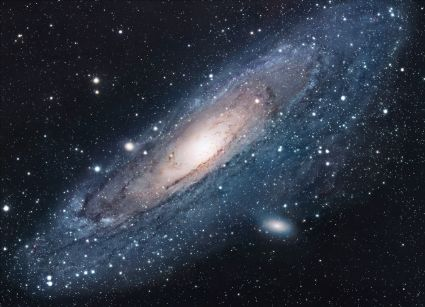
\includegraphics[scale=1.7]{universe.jpg}
\caption{The Universe}
\label{fig:universe}
\end{figure}

Many types of graphics images can be included, e.g., .png, .pdf, etc.  Make sure you upload your image to your project directory using the little arrow-to-cloud icon in the lower left of the ShareLaTeX site.

Another issue to be aware of with figures is the positioning argument.  In the universe example, we used \verb=\begin{figure}[h!]=, which forces the image to be located where inserted in the text.  Alternatively, the position argument can be omitted (leave off the square brackets) or you can use \verb=[t]= for top or \verb=[b]= for bottom of the page.  Keep in mind, however, that usually \LaTeX~is much better than you at figuring out where the figures should go and it is probably better to omit the position argument unless absolutely necessary.

Finally, note the scale optional argument in the \verb=\includegraphics= command.  A couple of useful options here are to directly specify the width and/or height of the image, e.g., \verb/[width=3.2in]/, or to specify the image width as a multiple of the page width, \verb/[width=.2\textwidth]/.  In Fig.~\ref{fig:smalluniverse} we show the result for the universe image using .2 scaled textwidth.

\begin{figure}
\centering
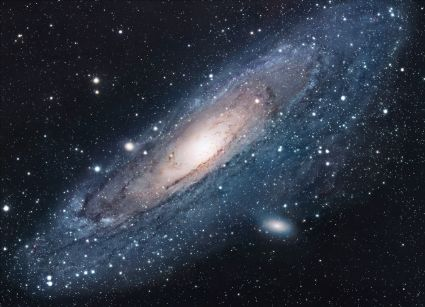
\includegraphics[width=0.2\textwidth]{universe.jpg}
\caption{The Small Universe}
\label{fig:smalluniverse}
\end{figure}

\subsection{Drawing Vector Graphics}

With the \href{http://www.texample.net/media/pgf/builds/pgfmanualCVS2012-11-04.pdf}{Ti\emph{k}Z drawing package} you can create your own vectorized (as opposed to rasterized) graphics.  This is especially helpful when the document may be resized (e.g., a poster) or used in a talk (with Beamer).  Below are two examples of the same image, one added with the \verb/\includegraphics/ command (Fig.~\ref{fig:raster}) from the previous section and one drawn with Ti\emph{k}Z (Fig.~\ref{fig:vector}).  View the PDF of this document and zoom in to high resolution to see the value of using vector graphics.

\begin{figure}[ht]
\begin{minipage}[c]{0.45\linewidth}
\centering
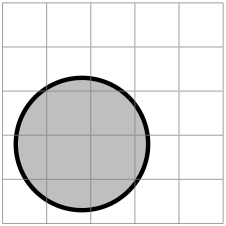
\includegraphics[width=.83\textwidth]{circle.png}
\caption{Raster image}
\label{fig:raster}
\end{minipage}
\hspace{0.5cm}
\begin{minipage}[c]{0.45\linewidth}
\centering
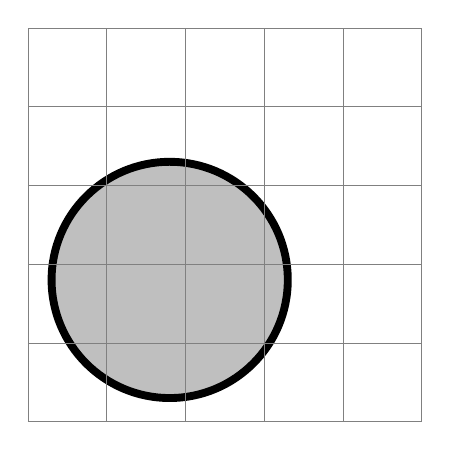
\begin{tikzpicture}
\draw[line width=1mm,fill=lightgray] (1.8,1.8) circle [radius=1.5];
\draw[help lines] (0,0) grid (5,5);
\end{tikzpicture}
\caption{Vector image}
\label{fig:vector}
\end{minipage}
\end{figure}

\section{Equations}

In this section, we provide examples for most of the equation constructs you will need in the class.  We start with symbols and work up to matrices.

\subsection{Symbols and Inline Math}

Most of the fancy symbols you will need are simply Greek names prefaced by a backslash, e.g., $\alpha$ is given by \verb=\alpha=.  If the equation is needed within the text, surround it by dollar signs, e.g., $y = mx + b$ is generated by \verb/$y=mx+b$/.  For the most part you do not need to worry about spacing in equations, though some fine-tuning may be required on occasion.  To slightly increase the space between symbols, add a \verb/\,/ \,. For example, $fg$ is produced by \verb/$fg$/, while $f\,g$ is produced by \verb/$f\,g$/.  To remove space use \verb/\!/ between symbols.

\subsection{Math Fonts in Figure Captions}

You want all math fonts to be consistent in your document whether they show up in an equation or in the main body of text or, as we will discuss here, in the text of a figure caption.  In Fig.~\ref{fig:example}, we plot an imaginary model comparison with data (the agreement is never this good!).  There are a few of points to make.  First, note that the fonts used for temperature, $T$, are consistent in this text, in the plot $y$-axis label, \emph{and} in the figure caption.  Next, notice that the font for the units, Kelvins, is K, not $K$ (this is discussed further in the next subsection). Last, note that you can (and should) use the figure caption to say something important about the figure.  If the figure does not convey an important point, why is it there to begin with?  Often, readers simply scan a paper and look at the plots or figures.  So, use this opportunity to communicate with your reader.  Draw them in and get them to read more detail in the text.

\begin{figure}
\centering
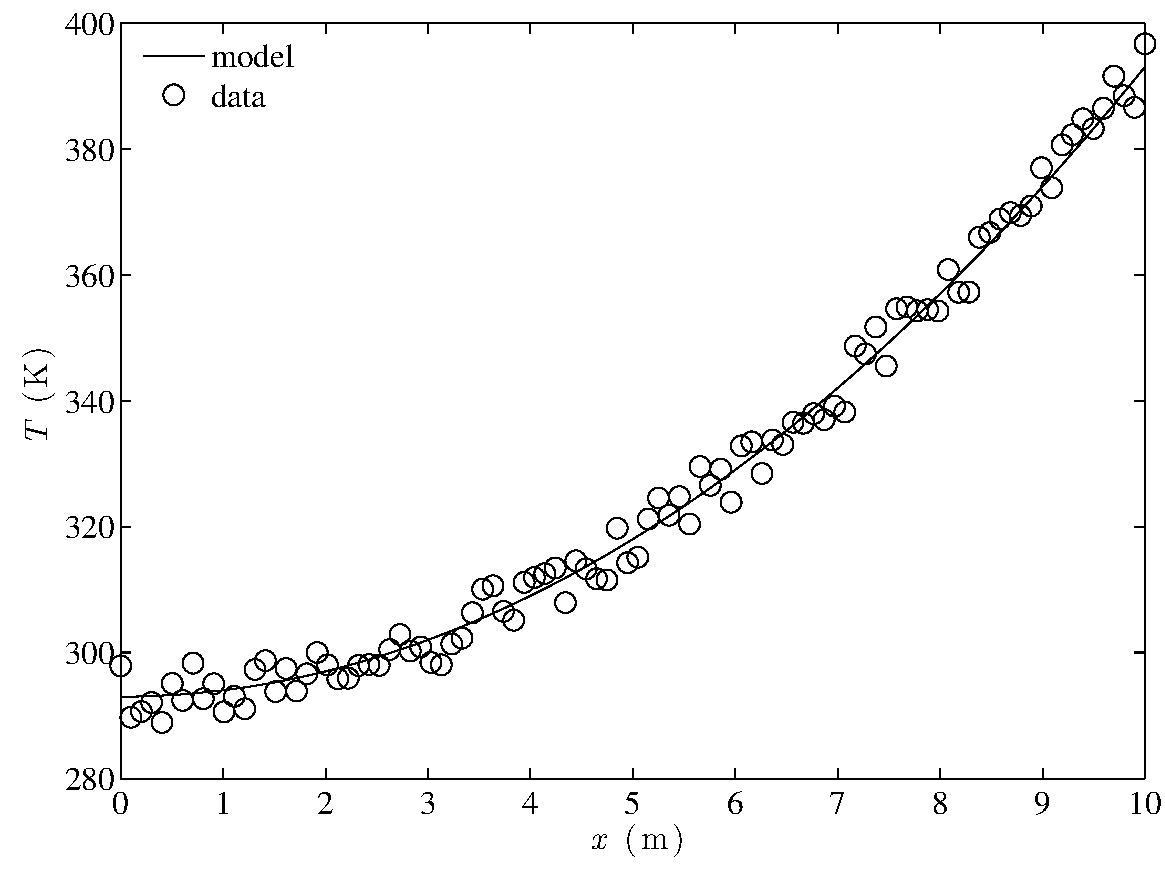
\includegraphics[width=0.75\textwidth]{example.pdf}
\caption{Model comparison with experimental data of axial profile of temperature, $T(x)$.  The agreement is remarkably good because this is a made up example.  This caption is a good place to tell the reader something important about the figure.  Often readers simply scan documents and look at the figures.  This is your chance to communicate the key result to the reader.  Don't waste the opportunity by being lazy and simply writing ``$T$ vs.~$x$''!}
\label{fig:example}
\end{figure}

\subsection{Units}

Units are generally not italicized.  The formal rules for what should and should not be italicized are documented in the \href{http://www.nist.gov/pml/pubs/sp811/index.cfm}{NIST Guide to SI Units} \cite{Thompson:2008}.  It is helpful to add \verb/usepackage{siunitx}/ to the preamble.  This allows you to easily include symbols, superscripts, etc., to units in the proper SI fonts, whether in math mode or not.

For example, if you want to write $T=20\,\si{\degree C}$, you would do this by \verb/$T=20\,\si{\degree C}$/. Below is a table of common unit problems with solutions using \verb/siunitx/.

\begin{center}
\begin{tabular}{ll}
unit & \verb/\si syntax/ \\
\hline
\si{m^2} & \verb/\si{m^2}/ \\
\si{kg m/s^2} & \verb=\si{kg m/s^2}= \\
\si{J/(m^2.s)} & \verb=\si{J/(m^2.s)}= \\
\si{J/(kg.\degree C)} & \verb=\si{J/(kg.\degree C)}=
\end{tabular}
\end{center}

\subsection{Numbering Equations}

As with sections, one of the most powerful features of \LaTeX~is the ability to reference equations.  Most of the time you will create equations using the \emph{equation environment} as follows:
\begin{equation}
\label{eq:line}
y = mx + b
\end{equation}
Now you can reference Eq.~(\ref{eq:line}) any time using \verb/\ref{eq:line}/.

You can also omit the equation number by using the \emph{displaymath envinronment}:
\begin{displaymath}
x = \frac{-b \pm \sqrt{b^2-4ac}}{2a}
\end{displaymath}

\subsection{Differential Equations and Integrals}

Here is an example of an ODE:
\begin{equation}
\label{eq:ode}
\frac{\d \mathbf{u}_p}{\d t} = \frac{1}{2}\rho\,C_d A_p (\mathbf{U}-\mathbf{u}_p)|\mathbf{U}-\mathbf{u}_p|
\end{equation}
Note that the differential operator is written as a Roman d, because $d$ is too often needed as a variable name, as in $diameter$.

Here is an example PDE:
\begin{equation}
\label{eq:pde}
\frac{\partial \rho}{\partial t} + \nabla\!\cdot(\rho \mathbf{u}) = 0
\end{equation}

Here is an example integral:
\begin{equation}
\label{eq:filter}
\int_a^b f(x) \,\d x = F(a) - F(b)
\end{equation}

\subsection{Equation Arrays}
In homework assignments it may often be necessary to show the development of an equation.  The \emph{align environment} is useful for this.  For example:
\begin{align}
f(x,y,z) &= (a + x)(b + y)(c + z) \notag\\
         &= (ab + ay + xb + xy)(c + z) \notag\\
         &= abc + ayc + xbc + xyc + abz + ayz + xbz + xyz
\end{align}
Notice that the equation number for the first two lines is suppressed using \verb/\notag/.  The anpersand \verb/&/ is used to set the alignment.  The \verb/\\/ is a carriage return.

\subsection{Matrices}
Matrices are created using the \verb/array/ environment within an \verb/equation/ environment.  The key trick here is to also use the \verb/\left/ and \verb/\right/ bracket commands which automatically size themselves to handle multiple rows or fractions.

\begin{equation}
\label{eq:matrix}
\mathsf{T} = \left( \begin{array}{ccc} \tau_{11} & \tau_{12} & \tau_{13} \\
                                       \tau_{21} & \tau_{22} & \tau_{23} \\
                                       \tau_{31} & \tau_{32} & \tau_{33} \end{array} \right)
\end{equation}

\section{Lists}
\label{sec:lists}

To make numbered or bulleted lists, use the \verb/enumerate/ or \verb/itemize/ environments.  Steps in an algorithm might be nicely described using
\begin{enumerate}
\item Compute the density
\item Compute the velocity
\item Solve the Poisson equation
\end{enumerate}
The ingredients in a recipe might be listed as
\begin{itemize}
\item 2 eggs
\item 1 cup of flour
\item 2 Tsp.~of cinnamon
\end{itemize}

\section{Bibliographic References}
\label{sec:bib_ref}

As with figure and equation references, \LaTeX provides a powerful means of citing references that makes life incredibly easy.  A database of references is stored in one or more \verb/.bib/ files.  Near the end of the document, the bib style and bib file are called (see the end of this \verb/main.tex/ file). The file \verb/references.bib/ is included with this template and contains a few examples.  Within the text, citations are refenced by the name assigned in the \verb/.bib/ file, for example, \cite{FDS_Math_Guide}.  More than one citation can be referenced at a time \cite{Beyler:hood,FDS_Math_Guide}.

You may add as many references to the \verb/references.bib/ file as you like.  Only the references specifically called out with a \verb/\cite{}/ command will be added to the {\bf References} section at the end of the document.  I encourage you to grow your own \verb/.bib/ database for use throughout your career.  As a good starting point, the database for the FDS manuals contains most of the papers relevant to fire dynamics:

\vskip\baselineskip
\noindent{\small\tt\url{http://code.google.com/p/fds-smv/source/browse/trunk/FDS/trunk/Manuals/Bibliography/FDS_general.bib}}

\section{Compiling Outside ShareLaTeX}

If you choose not to use the ShareLaTeX site, you need to know how to compile the document.  In order to resolve all the cross-referencing in the \verb/\cite{}/ and \verb/\ref{}/ calls, you must run \verb/pdflatex/ and \verb/bibtex/ in the following order:
\begin{enumerate}
\item \verb/pdflatex/
\item \verb/bibtex/
\item \verb/pdflatex/
\item \verb/pdflatex/
\end{enumerate}

In the process, \LaTeX will create several inermediate files that it uses to get itself from one stage to the next.  If you are using Windows, I recommend using the MikTeX distribution and also using the trial version of WinEdt.  Once installed, you can simply click a few icons to compile the document.  On a Mac, TeXShop contains pretty much everything you need.

\section{Spell Checking}

Most editors have a spell checker.  But it is not a prerequisite for \LaTeX, so be careful.

\section{Conclusion}

Congratulations. If you have made it this far, you are on your way to becoming a \LaTeX~guru and watching sympathetically as your colleagues waste hours rearranging figures and references and search through ``objects'' to ``insert'' into equations that ultimately look amateurish.  You may now focus on content, and leave the formatting to the pros.

\begin{quotation}
``I always thought something was fundamentally wrong with the universe'' \cite{adams1995hitchhiker}
\end{quotation}

\section*{Acknowledgments}

I'd like to thank The Academy.

\appendix

\section{Appendices}

The appendices come before the references.  Use the \verb/\section/ command to start a new appendix.

\bibliographystyle{plain}
\bibliography{references}
\end{document}
